%%%%%%%%%%%%%%%%%%%%%%%%%%%%%%%%%%%%%%%%%
% Wenneker Article
% LaTeX Template
% Version 2.0 (28/2/17)
%
% This template was downloaded from:
% http://www.LaTeXTemplates.com
%
% Authors:
% Vel (vel@LaTeXTemplates.com)
% Frits Wenneker
%
% License:
% CC BY-NC-SA 3.0 (http://creativecommons.org/licenses/by-nc-sa/3.0/)
%
%%%%%%%%%%%%%%%%%%%%%%%%%%%%%%%%%%%%%%%%%

%----------------------------------------------------------------------------------------
%	PACKAGES AND OTHER DOCUMENT CONFIGURATIONS
%----------------------------------------------------------------------------------------

\documentclass[10pt, a4paper, twocolumn]{article} % 10pt font size (11 and 12 also possible), A4 paper (letterpaper for US letter) and two column layout (remove for one column)

%%%%%%%%%%%%%%%%%%%%%%%%%%%%%%%%%%%%%%%%%
% Wenneker Article
% Structure Specification File
% Version 1.0 (28/2/17)
%
% This file originates from:
% http://www.LaTeXTemplates.com
%
% Authors:
% Frits Wenneker
% Vel (vel@LaTeXTemplates.com)
%
% License:
% CC BY-NC-SA 3.0 (http://creativecommons.org/licenses/by-nc-sa/3.0/)
%
%%%%%%%%%%%%%%%%%%%%%%%%%%%%%%%%%%%%%%%%%

%----------------------------------------------------------------------------------------
%	PACKAGES AND OTHER DOCUMENT CONFIGURATIONS
%----------------------------------------------------------------------------------------

\usepackage[english]{babel} % English language hyphenation

\usepackage{microtype} % Better typography

\usepackage{amsmath,amsfonts,amsthm} % Math packages for equations

\usepackage[svgnames]{xcolor} % Enabling colors by their 'svgnames'

\usepackage[hang, small, labelfont=bf, up, textfont=it]{caption} % Custom captions under/above tables and figures

\usepackage{booktabs} % Horizontal rules in tables

\usepackage{lastpage} % Used to determine the number of pages in the document (for "Page X of Total")

\usepackage{graphicx} % Required for adding images

\usepackage{enumitem} % Required for customising lists
\setlist{noitemsep} % Remove spacing between bullet/numbered list elements

\usepackage{sectsty} % Enables custom section titles
\allsectionsfont{\usefont{OT1}{phv}{b}{n}} % Change the font of all section commands (Helvetica)

%----------------------------------------------------------------------------------------
%	MARGINS AND SPACING
%----------------------------------------------------------------------------------------

\usepackage{geometry} % Required for adjusting page dimensions

\geometry{
	top=1cm, % Top margin
	bottom=1.5cm, % Bottom margin
	left=2cm, % Left margin
	right=2cm, % Right margin
	includehead, % Include space for a header
	includefoot, % Include space for a footer
	%showframe, % Uncomment to show how the type block is set on the page
}

\setlength{\columnsep}{7mm} % Column separation width

%----------------------------------------------------------------------------------------
%	FONTS
%----------------------------------------------------------------------------------------

\usepackage[T1]{fontenc} % Output font encoding for international characters
\usepackage[utf8]{inputenc} % Required for inputting international characters

\usepackage{XCharter} % Use the XCharter font

%----------------------------------------------------------------------------------------
%	HEADERS AND FOOTERS
%----------------------------------------------------------------------------------------

\usepackage{fancyhdr} % Needed to define custom headers/footers
\pagestyle{fancy} % Enables the custom headers/footers

\renewcommand{\headrulewidth}{0.0pt} % No header rule
\renewcommand{\footrulewidth}{0.4pt} % Thin footer rule

\renewcommand{\sectionmark}[1]{\markboth{#1}{}} % Removes the section number from the header when \leftmark is used

%\nouppercase\leftmark % Add this to one of the lines below if you want a section title in the header/footer

% Headers
\lhead{} % Left header
\chead{\textit{\thetitle}} % Center header - currently printing the article title
\rhead{} % Right header

% Footers
\lfoot{} % Left footer
\cfoot{} % Center footer
\rfoot{\footnotesize Page \thepage\ of \pageref{LastPage}} % Right footer, "Page 1 of 2"

\fancypagestyle{firstpage}{ % Page style for the first page with the title
	\fancyhf{}
	\renewcommand{\footrulewidth}{0pt} % Suppress footer rule
}

%----------------------------------------------------------------------------------------
%	TITLE SECTION
%----------------------------------------------------------------------------------------

\newcommand{\authorstyle}[1]{{\large\usefont{OT1}{phv}{b}{n}\color{DarkRed}#1}} % Authors style (Helvetica)

\newcommand{\institution}[1]{{\footnotesize\usefont{OT1}{phv}{m}{sl}\color{Black}#1}} % Institutions style (Helvetica)

\usepackage{titling} % Allows custom title configuration

\newcommand{\HorRule}{\color{DarkGoldenrod}\rule{\linewidth}{1pt}} % Defines the gold horizontal rule around the title

\pretitle{
	\vspace{-30pt} % Move the entire title section up
	\HorRule\vspace{10pt} % Horizontal rule before the title
	\fontsize{32}{36}\usefont{OT1}{phv}{b}{n}\selectfont % Helvetica
	\color{DarkRed} % Text colour for the title and author(s)
}

\posttitle{\par\vskip 15pt} % Whitespace under the title

\preauthor{} % Anything that will appear before \author is printed

\postauthor{ % Anything that will appear after \author is printed
	\vspace{10pt} % Space before the rule
	\par\HorRule % Horizontal rule after the title
	\vspace{20pt} % Space after the title section
}

%----------------------------------------------------------------------------------------
%	ABSTRACT
%----------------------------------------------------------------------------------------

\usepackage{lettrine} % Package to accentuate the first letter of the text (lettrine)
\usepackage{fix-cm}	% Fixes the height of the lettrine

\newcommand{\initial}[1]{ % Defines the command and style for the lettrine
	\lettrine[lines=3,findent=4pt,nindent=0pt]{% Lettrine takes up 3 lines, the text to the right of it is indented 4pt and further indenting of lines 2+ is stopped
		\color{DarkGoldenrod}% Lettrine colour
		{#1}% The letter
	}{}%
}

\usepackage{xstring} % Required for string manipulation

\newcommand{\lettrineabstract}[1]{
	\StrLeft{#1}{1}[\firstletter] % Capture the first letter of the abstract for the lettrine
	\initial{\firstletter}\textbf{\StrGobbleLeft{#1}{1}} % Print the abstract with the first letter as a lettrine and the rest in bold
}

%----------------------------------------------------------------------------------------
%	BIBLIOGRAPHY
%----------------------------------------------------------------------------------------

\usepackage[backend=bibtex,style=authoryear,natbib=true]{biblatex} % Use the bibtex backend with the authoryear citation style (which resembles APA)

\addbibresource{example.bib} % The filename of the bibliography

\usepackage[autostyle=true]{csquotes} % Required to generate language-dependent quotes in the bibliography
 % Specifies the document structure and loads requires packages
\newcommand{\specialcell}[2][c]{%
  \begin{tabular}[#1]{@{}c@{}}#2\end{tabular}}
%----------------------------------------------------------------------------------------
%	ARTICLE INFORMATION
%----------------------------------------------------------------------------------------

\title{Vision Team Project Proposal :\\ What the hell is that ?} % The article title

\author{
	 \textbf{Email Team} : vision@chalearn.org \\
	 \textbf{Team} :
	 Vincent BOYER	\emph{[vincent.boyer1@live.fr]};
	 \: Ludovic KUN	\emph{[kun.ludovic@yahoo.fr]};\\
	  Qixiang PENG	\emph{[kevin.pqx@icloud.com]};
	 \: Perceval WAJSBURT	\emph{[perceval.wajsburt@gmail.com]};\\
	 Warren PONS	\emph{[warren.pons@hotmail.fr]}\\
	 \textbf{Github }: \emph{https://github.com/vincentBoyer1/VISION\_project}
	%\authorstyle{No one\textsuperscript{1,2,3} and One No\textsuperscript{2,3}} % Authors
	%\newline\newline % Space before institutions
	% vision@chalearn.org
	%\textsuperscript{1}\institution{ vision@chalearn.org}\\ % Institution 1
	%\textsuperscript{2}\institution{University of Texas at Austin, Texas, United States of America}\\ % Institution 2
	%\textsuperscript{3}\institution{\texttt{LaTeXTemplates.com}} % Institution 3
}

% Example of a one line author/institution relationship
%\author{\newauthor{John Marston} \newinstitution{Universidad Nacional Autónoma de México, Mexico City, Mexico}}

\date{\today} % Add a date here if you would like one to appear underneath the title block, use \today for the current date, leave empty for no date

%----------------------------------------------------------------------------------------
\usepackage{float}
\begin{document}

\maketitle % Print the title

\thispagestyle{firstpage} % Apply the page style for the first page (no headers and footers)

%----------------------------------------------------------------------------------------
%	ABSTRACT
%----------------------------------------------------------------------------------------



%----------------------------------------------------------------------------------------
%	ARTICLE CONTENTS
%----------------------------------------------------------------------------------------

\section{Background}
%\citep{}
\lettrineabstract{Since the end of the 20th century, autonomous vehicles have been debated within the scientific community. Combining artificial intelligence and industrial know-how, they are one of the major objectives of the beginning of the 21th century. We can note for example the GoogleCar project, the Testla Autopilot or the AVA(Autonomous Vehicle for All) project from PSA. However, obstacles remain to be overcome, in particular the behavior of the vehicle in response to its environment of evolution. This step is based on the analysis of its environment and therefore on the entities that make it up. In this challenge, we will therefore study the preliminary stage of the Decision, ie the classification of the detected entities (by the cameras of the vehicle for example). To illustrate this problematic, we propose to study the image source CIFAR-10 which groups entities that can interact with the vehicle environment like animals(cat, horse, dog, ...) and vehicles (bike, car, truck, ...).
%With the development of automatic  transport means (trains, cars, boats, ...), it is necessary to identify the elements detected by the cameras in order to act accordingly. Indeed, the device will not act in the same way if it detects a frog or if it detects a horse for example. The idea of this project is to be able to detect entities that can be found when traveling by rail, sea or road. The recognition of these entities is therefore essential if we want to achieve intelligent and safe autonomous transport.
%Avec le développement des moyens de transports automatiques(trains, voitures, bateaux, ...), il est nécessaire d'identifier les éléments détectes par les caméras afin de pouvoir agir en conséquence. En effet, l'appareil n'agira pas de la même manière s'il detecte une grenouille ou s'il detecte un cheval par exemple.  L'idée de ce projet est d'être capable de détecter des entitées que l'on peut retrouver lors de trajet ferroviaire, maritime ou bien routier. La reconnaissance de ces entitées est ainsi primordiale si l'on veut pouvoir réaliser des transports autonomes intelligents et sûres.%% 
}

%------------------------------------------------



%------------------------------------------------

\section{Material and Methods}

\subsection{Data description}
The dataset used for this project is CIFAR10 [\cite{1}](Figure \ref{fig:cifar10}) which is composed of 60 000 images of size 32 x 32 representing 10 labels of animals and means of transport.  The datasets is divided as follows: 40 000 for the training step, 10 000 for the testing step and 10 000 for the validation step. Each set is balance distributed (Table~\ref{tab1}).
\begin{table}
\begin{tabular}{|l|c|c|c|c|}
  \hline
  Labels & Train & Test & Validation & Total\\
  \hline
  airplane & 4000 & 1000 & 1000 & 6000 \\
  \hline
  automobile & 4000 & 1000 & 1000 & 6000\\
  \hline
  bird & 4000 & 1000 & 1000 & 6000\\
  \hline
  cat & 4000 & 1000 & 1000 & 6000\\
  \hline
  deer & 4000 & 1000 & 1000 & 6000\\
  \hline
  dog & 4000 & 1000 & 1000 & 6000\\
  \hline
  frog & 4000 & 1000 & 1000 & 6000\\
  \hline
  horse & 4000 & 1000 & 1000 & 6000\\
  \hline
  ship & 4000 & 1000 & 1000 & 6000 \\
  \hline
  truck & 4000 & 1000 & 1000 & 6000\\
  \hline
  Total & 40000 & 10000 & 10000 & 60000\\
  \hline
\end{tabular}
\caption{\label{tab1} Distribution of each set : train, validation, set}
\end{table}


\subsection{Preprocessing}
Before classifying the different images of our dataset, we need to preprocess the images, extracting the features, which will permits us to classify them more precisely. In fact, classifying directly the images will gives us bad results (Table \ref{tab2}), which is why extract features are necessarily.  Different features are used like HoG (Histogram of Gradient) available on the library skilage in python but the result is pretty bad (Table \ref{tabHOG}). So we decide to use convolutional neural network used in Deep Learning [\cite{2}].  We use the MobileNet [\cite{3}] architecture of Google on the Keras Framework, and we added some layers so as to reduce the size of the features to 256. We do not want to take features bigger than 256 because the computation time will increase for the different algorithm of classification. We do not want to reduce too much the features because we want to let the possibility for the student to try to reduce the dimension of the dataset.  Regarding the architecture, MobileNet is a good feature extractor because it is a fast and soft model (so our personal computer is powerful enough) with a good accuracy on ImageNet. This is why we use it. We save 256 features for each image in CIFAR10 in the AutoML format. 

\subsection{Method}
We consider our problem as a multi label classification therefore each image is associated to a label value between 0 and 9 included. The final step is to use a machine learning algorithm(using skicit learn for example) so as to be able to predict the class of an image. There are a lot of machine learning algorithm permitting to solve this problem so student have to classify the features with different models and choose the best they obtain. (Naives bayes, SVM, tree, …).
If the student is familiar with the keras framework, he/she can also classify features with a simple neuronal network ! \\The set of data (features) have 256 dimensions and can be subject to a reduction of dimension in order to limit the training time of the models and to limit the difficulty associated to the Curse of Dimensionality. As we can see on the figure \ref{fig:graph_1}, using  principal component analysis (PCA), it is possible to lessen the number of features (about $73\%$ is conserved keeping only 10 dimensions, and about $80\%$ is conserved keeping only 20 dimensions). The reduction of dimension is an important pre-processing step and even if it is not essential to get
results on this dataset, it permits to save learning time on model which is non-negligible.
\\

\begin{table}[H]
\hspace{-1.0 cm}
\begin{tabular}{|l|c|c|c|c|}
  \hline
  Model & Accuracy & Recall & Precision & F1\\
  \hline
  Tree & 0.22 & 0.22 & 0.22 & 0.22\\
  \hline
  Random Forest & 0.21 & 0.20 & 0.21 & 0.15\\
  \hline
  \specialcell{Naives Bayes \\Gaussian} & \textbf{0.27} & \textbf{0.28} & \textbf{0.27} & \textbf{0.25}\\
  \hline
  \specialcell{Naives Bayes \\ Multinomial} & 0.24 & 0.25 & 0.24 & 0.22\\
  \hline
\end{tabular}
\caption{\label{tab2}Classification's result without extraction features}
\end{table}

\begin{table}[H]
\hspace{-1.0 cm}
\begin{tabular}{|l|c|c|c|c|}
  \hline
  Model & Accuracy & Recall & Precision & F1\\
  \hline
  Tree & 0.254 & 0.254 & 0.254 & 0.254\\
  \hline
  Random Forest & 0.2819 & 0.314 & 0.2819 & 0.231\\
  \hline
  \specialcell{Naives Bayes \\Gaussian} & \textbf{0.4308} & \textbf{0.4315} & \textbf{0.4308} & \textbf{0.421}\\
  \hline
  \specialcell{Naives Bayes \\ Multinomial} & 0.4095 & 0.412 & 0.4095 & 0.4048\\
  \hline
  \specialcell{SVM RBF} & 0.2698 & 0.353 & 0.2698 & 0.235\\
  \hline
\end{tabular}
\caption{\label{tabHOG}Classification's result using HoG as extraction features}
\end{table}
\begin{figure}[H]
	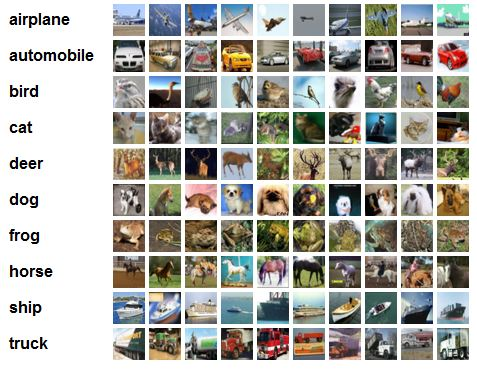
\includegraphics[width=\linewidth]{cifar10.jpg} % Figure image
	\caption{\label{fig:cifar10}Representation of the dataset Cifar10}
\end{figure}
\section{Preliminary results}
In this experiment, we tested differents models and compared their performance (Table \ref{tab3}, \ref{tab4}). The different metric used to determine the performance of our models are : accuracy, accuracy per class, recall, precision, F1-score. We could also used the balanced accuracy metric instead of the regular accuracy but all class of the set are homogenous distributed (same numbers of examples per class) so the result is the same. We note that SVMs models are very efficient on the features extracted by the convolutional neural network and more accuracy equilibrate regarding the accuracy per class (cf Table \ref{tab4}) but it takes some time to construct the model contrary to the others models like tree or random forest which have lowest performances but they are faster to learn. We can also note that tree and random forest have more difficulty predict well a cat contrary to the others models (cf Table \ref{tab4}).  However, the computing time of the prediction is pretty fast for all the models.


\begin{table}[!h]
\hspace{-0.3cm}
\begin{tabular}{|l|c|c|c|c|c|}
  \hline
  Model & Accuracy & Recall & Precision & F1 & \specialcell{Time \\(sec)}\\
  \hline
  Tree & 0.797 & 0.798 & 0.797 & 0.797 & 16.73\\
  \hline
  \specialcell{Random\\ Forest} & 0.831 & 0.829 & 0.831 & 0.830 & 33.42\\
  \hline
  \specialcell{Naives Bayes \\Gaussian} & 0.853 & 0.856 & 0.853 & 0.854 & 0.198\\
  \hline
  \specialcell{Naives Bayes \\ Multinomial} & 0.866 & 0.869 & 0.866 & 0.867 & \textbf{0.06}\\
  \hline
   SVM rbf &\textbf{ 0.888} & \textbf{0.888} & \textbf{0.888} & \textbf{0.888} & 87.49\\
   \hline
   SVM Linear & 0.871 & 0.872 & 0.871 & 0.872 & 173.15\\
   \hline
   SVM Poly & 0.886 & 0.887 & 0.886 & 0.886 & 66.24\\
   \hline
\end{tabular}
\caption{\label{tab3}Classification's result with extraction features on the test set}
\end{table}

\begin{table}[!h]                         
\hspace{-0.3cm}
\begin{tabular}{|l|c|c|c|c|c|c|c|}                   
  \hline
  Class & Tree  & \specialcell{Random\\ Forest} & \specialcell{Naives Bayes \\Gaussian}& \specialcell{Naives Bayes \\ Multinomial} & SVM rbf  & SVM Linear & SVM Poly\\
  \hline
   airplane & 0.821  & 0.834 & 0.907 & 0.924 & 0.925 & 0.893 & 0.918 \\
  \hline
   automobile &  0.906 & 0.93 & 0.936 & 0.956 & 0.952 & 0.941 & 0.957\\
  \hline
   bird & 0.732 & 0.761 & 0.756 & 0.825 & 0.849 & 0.842 & 0.85 \\
  \hline
   cat & 0.64 & 0.606 & 0.772 & 0.832 & 0.795 & 0.779 & 0.819\\
  \hline
  deer & 0.747 & 0.774 & 0.825 & 0.861 & 0.871 & 0.856 & 0.875 \\
   \hline
    dog & 0.73 & 0.796 & 0.76 & 0.768 & 0.795 & 0.786 & 0.773\\
   \hline
    frog & 0.856 & 0.915 & 0.882 & 0.913 & 0.924  & 0.914 & 0.918 \\
    \hline
	horse & 0.79 & 0.851 & 0.847 & 0.877 & 0.899 & 0.87 & 0.878 \\
	\hline
	ship & 0.871 & 0.916 & 0.921 & 0.942 & 0.936 & 0.923 & 0.937 \\
	\hline
	truck & 0.884 & 0.933 & 0.925 & 0.956 & 0.937 & 0.915 & 0.935 \\
   \hline
\end{tabular}
\caption{\label{tab4} Accuracy per class with CNN extraction features on the test set}
\end{table}
The results associated with the learning on the data processed by PCA are available on the
figure \ref{fig:graph_1}. As we can see, performances are very similar to learning on the initial features (see table \ref{tab3} and figure \ref{fig:graph_1}) when the dimension is superior to 10. The use of PCA (or other method of reducing
dimension) is left to the student's sensitivity because this stage of pre-processing is a matter of
good understanding about how to learn a dataset. However this step is  not mandatory considering the potential lacking experience of the student.
\begin{figure}[H]
\center
	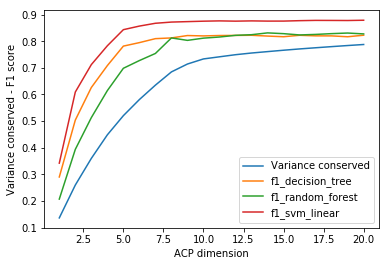
\includegraphics[scale=0.4]{graph_1.png} % Figure image
	\caption{\label{fig:graph_1}Graph representing F1 score depending of the number of dimension} % Figure caption
	 % Label for referencing with \ref{bear}
\end{figure}

\begin{figure}[H]
\center
	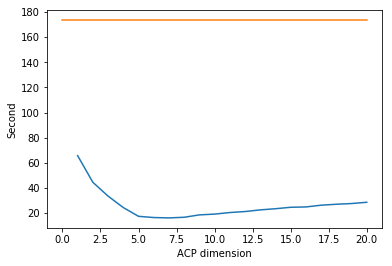
\includegraphics[scale=0.4]{graph_2.png} % Figure image
	\caption{\label{fig:graph_2}Graph representing the training time depending of the number of dimension. In blue, the training time of the SVM linear model depending of the number of features, in orange the training time of the SVM linear on the original features(256)} % Figure caption
	 % Label for referencing with \ref{bear}
\end{figure}
%----------------------------------------------------------------------------------------
%	BIBLIOGRAPHY
%----------------------------------------------------------------------------------------


\vspace*{6cm}
\begin{thebibliography}{abcde}

	\bibitem[1]{cifar} https://www.cs.toronto.edu/~kriz/cifar.html\\
    \bibitem[2]{convnet} "CNN Features off-the-shelf: an Astounding Baseline for Recognition", Ali Sharif Razavian et al, 2014.
 
    \bibitem[3]{mobilenet} "MobileNets: Efficient Convolutional Neural Networks for Mobile Vision Applications" ,Andrew G. Howard, Menglong Zhu et al, 2017.
\end{thebibliography}
%\printbibliography[title={Bibliography}] % Print the bibliography, section title in curly brackets

%----------------------------------------------------------------------------------------

\end{document}
